\documentclass[12pt]{article}
\usepackage{graphicsx}
\graphicspath{{images/}}
\usepackage{sidecap}

% Title Page
\title{PIC16F684 Line-Following Robot}
\author{Dar Mehta}
\date{January 15, 2015}


\begin{document}
\maketitle
\newpage
\tableofcontents
\newpage

\section{Abstract}	
The robot is designed to follow a specified black line made out of electrical tape on a white surface. The programming was done using the assembly language on the PIC 16F684 microcontroller (herein referred to as PIC microcontroller), whereas the motor control was handled by the L293DNE chip.
\\[\baselineskip]
This report details the design and development of the line following robot including the purpose, materials and the initial and final designs of the robot. The construction of the robot involved the mounting of two light sensors, the PIC microcontroller and a breadboard for the circuit onto a pre-built robot chassis. Furthermore, this report also includes a detailed step-by-step construction of the robot that the reader can follow to recreate the robot. Lastly, the report includes problem diagnosis stating the description and root cause, symptoms, and solutions and design changes. The appendix includes layout diagrams of the robot and the circuit as well as pictures of the final robot, program flowchart, the final code and links to datasheets for the components used are located in the appendix.

\section{Objective}
The objective of this project, as assigned in class, is to build an autonomous line following robot using the PIC microcontroller and light sensors. The two light sensors are used to allow the robot to detect a black line on a white surface while the L293DNE controls the movement of the robot.
\\[\baselineskip]
The original goal of the robot was to use an algorithm that will keep the robot centred on the black line while it completes one lap of a track outlined with black electrical tap on a white surface in 60 seconds. However, midway through the project, due to technical difficulties combined with time constraints, the goal was changed so that the robot is using a hardcoded algorithm that will allow the robot to complete the track from point A to point B in 45 seconds. In these 45 seconds, the robot must start at one end of the course, reach the other end, and come to a complete stop at the end of the track.

\section{Components}
\subsection{PIC16F684 Microcontroller}
The Peripheral Interface Controller is a chip consisting of 14 pins and will be used as the “brain” of the robot in order to control its motors and sensors. A program is written in assembly on a compatible IDE such as MP LAB. It is then built, compiled and uploaded by the IDE to the microcontroller. This program is run by applying +5V of power to the chip. The pins on the controller can be configured for output or input in order to either control a device such has a motor or read data from a device such as a light sensor, respectively.

\subsection{L293DNE Motor Controller}
The L293DNE motor controller has 16 pins and is connected to each of the two motors. It is also connected to the PIC Microcontroller in order to be able to control the start/stop and direction of each motor. Pins 1, 8, 9, and 16 are connected to the power supply via an LM7805 Voltage Regulator which provides 5V. Pins 4, 5, 12 and 13 are grounded. Motor 1 is connected to pins 3 and 6 and is controlled by pins 2 and 7. Motor 2 is connected to pins 11 and 14 and is controlled by pins 10 and 15. Pins 2, 7, 10 and 15 which control the two motors are connected to the output pins on the PIC microcontroller. See data sheet in references section below for more details.

\subsection{LM7805 Voltage Regulator}
The LM7805 voltage regulator is connected to the robot’s circuit in order to ensure no components are damaged due to excess voltage. It consists of three pins: an input which takes in any input voltage, a ground, and an output which outputs a safe voltage of 5V.

\subsection{QRD1114 Sensors (x2)}
The QRD1114 is a light sensor consisting of four pins - a cathode, an anode, an emitter and a collector. Refer to the datasheet in the references section below for more details about each of the four pins. The sensor emits infrared light that is powered constantly and detects the reflectivity of this emitted light. Typically, the darker the surface, the more the light is absorbed and so less light is detected by the phototransistor. When light is detected by the phototransistor, current flows through the sensor thus sending an analog signal to the PIC microcontroller. This allows the sensor to differentiate between black and white surfaces.

\subsection{Breadboard}
A breadboard is used for easy construction and debugging of the robot’s circuit as it requires no soldering.

\section{Design}
\subsection{Code}
\begin{enumerate}
	\item Set PORTA pins RA0, RA1, RA4, RA5 as output.
	\item Set PORTC pins RC0 and RC1 to input (AN4 and AN5 = 1). \item Set up AN4 and AN5 as analog inputs using ANSEL.
	\item Set the internal clock (ADCON1 = 00110000).
	\item Set ADCON0.
	\begin{enumerate}
		\item The ADRES value should be left-justified.
		\item The voltage reference should be the VDD pin.
		\item The analog channel should initially be set to AN5. d. The GO/DONE bit should be cleared.
		\item Enable the ADC.
	\end{enumerate}
\textit{Refer to page 70 of the PIC16F684 Data Sheet for more information on how to configure these registers.}

	\item Begin the main program loop.
	\item Save the ADRESH value.
	\item Set the analog channel to AN4 and repeat the procedure for the other sensor. 9. Compare the ADRES values to a threshold value.
	\item If the sensor sees white, turn the corresponding wheel, else stop the motor. 11. Repeat program indefinitely to continue reading sensors.
	
\textit{Refer to the attached document for the specific code used.}
\end{enumerate}

\subsection{Program Flowchart}
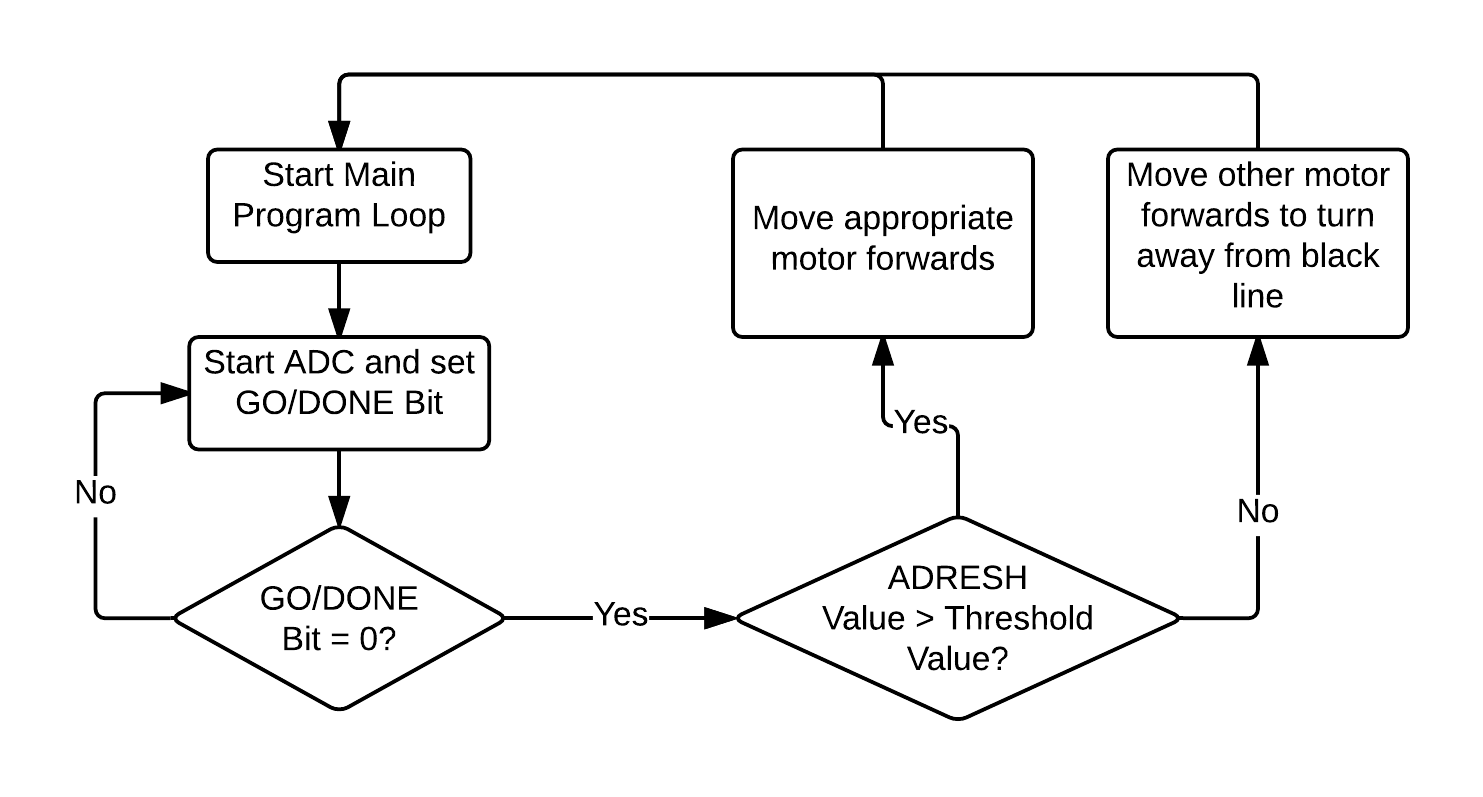
\includegraphics{ProgramFlowchart}
\subsection{Circuit}
\begin{enumerate}
	\item Build the motor controller circuit on the breadboard that came pre-attached with the robot chassis. Refer to appropriate datasheet and pictures in the appendix for more information.
	\item Connect both motors to the motor controller.
	\item On a different breadboard, construct the sensor circuitry. Use appropriate 10K and 320Ω resistors to avoid damage to the sensors. Refer to datasheet for detailed information regarding the use of correct resistors as to not damage the sensor.
	\item Ensure the use of a voltage regulator connected to both the motor controller circuit and the sensor circuitry.
	\item Connect an external power supply to power all the components - PIC microcontroller, sensors and L293DNE - with 5V through the voltage regulator.
	\item Connect the ground of all components - PIC microcontroller, sensors and L293DNE - to the ground of the power supply.

	
	\textit{Refer to the attached document for a full schematic of the motor controller circuit. The sensor circuit has been omitted as it was not used in the final design of the robot.}
\end{enumerate}

\subsection{Hardware}
\begin{enumerate}
	\item Using screws and brackets, attach the sensors 3.5 cm apart in width to allow it to straddle the line which is approximately 2 cm in width. This gives the robot approximately 0.75 cm on each side of the line to detect the white surface.
	\item Ensure they are approximately 2 mm above the ground to receive accurate readings from the sensors.
	\item Mount the sensors 1mm in front of the robot in order to ensure easy accessibility to the sensor wiring for debugging.
	\item Mount the breadboard containing the sensors circuitry onto the PIC microcontroller, as shown in pictures found in the appendix, using double sided tape. Then mount the entire PIC microcontroller and breadboard assembly on the top of the robot chassis with tape.
\end{enumerate}
\newpage
\section{Problem Diagnosis and Correction}
\begin{table} [h!]
	\centering
		\hspace*{-3cm}
		\resizebox{20cm}{!}{%
		\begin{tabular}{|p{5cm}|p{5cm}|p{8.5cm}|}
			\hline
			Problem Description & Symptoms & Solutions \& Design Changes \\
			\hline
			The robot only moved for 2 seconds before coming to a stop.
The root cause of this problem was improper circuitry design which didn't provide any external power to the L293DNE motor controller. & The wheels on the robot moved for 2 seconds and then halted to a stop. However, the motors continued to turn as the sound of the motor was clearly audible. Although it is not known with certainty, the worm gear may have been stripped as a result. & \textbf{Solution:} The solution was to provide more voltage through an AC/DC Wall Adapter. 

\textbf{Design Changes:} A LM7805 voltage regulator was added to the circuit in order to ensure that only 5V from the power source were applied to the L293DNE motor controller. This change was verified to be extremely effective as it solved the problem and ensured safe operation. \\
\hline
The left side of the robot wouldn’t move even though the motor was spinning as it was audible.
The root cause of this was that the worm gear of the motor was not aligned with the drive gear due to incorrect spacing between the two gears. & The incorrect spacing between the gears did not allow for the motor to transfer torque to the wheel. Thus, the robot spun in circles since only the right side wheels were spinning. & \textbf{Solution:} The drive gear was pushed upwards so that it was interlocked with the worm gear on the motor.

\textbf{Design Changes:} A screw was added to the bottom floor of the chassis to push the gear upwards. This solution was extremely effective as it solved the problem and in turn, allowed for the code to work effectively as the robot continued to move as expected.\\
\hline
The sensors had no impact on the robot’s decision making.
The root cause of this issue is the erroneous code in which the GO/DONE bit was not enabled in the ADC procedure. As such, the analog signal from the sensors were never being read as digital. & Due to the code not enabling the GO/DONE bit which caused the sensors t never be read, the robot continued to go straight off the track as if the sensors were always seeing white. & \textbf{Solution:} Originally, it was thought the sensors were faulty. They were replaced but despite not having any effect and the code having been checked by several peers, the origin of the problem could not be resolved. The issue was only noticed after an example code was shown by Mr. Balcita on the sue of ADC conversion.

\textbf{Design Changes} The robot was changed to use timed delays to hardcode its decision making process so that it would follow the preset track.Although extremely effective and quick, this design could have been avoided by being persistent with the light sensors.\\
			\hline
		\end{tabular}}
\end{table}
\newpage
\section{Conclusion}
The original objective was to construct a line following robot using the assembly language to program the PIC 16F684 microcontroller. The specifications indicated using light sensors to sense a black line on a white surface that will allow the robot to complete one lap of the track made out of black electrical tape in 60 seconds.
\\[\baselineskip]
The robot does not meet the original objective as it is able to move around the track but not complete a full lap on the track. Additionally, the robot uses a hardcoded assembly program instead of using light sensors to follow the line.
\newpage
\section{Appendix}
	\begin{SCfigure}[0.5][h]
		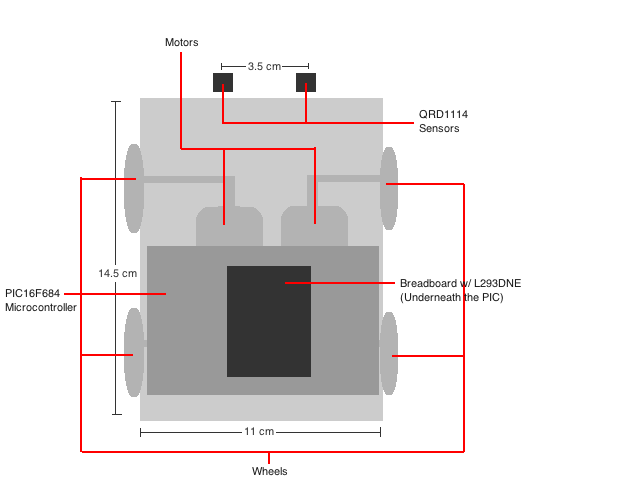
\includegraphics[width=10cm]{LayoutDiagram}
		\caption{The final robot layout is shown to the left. The motor controller circuit is mounted beneath the PIC16F684 Microcontroller.}
	\end{SCfigure}
	\begin{SCfigure}[0.5][h!]
	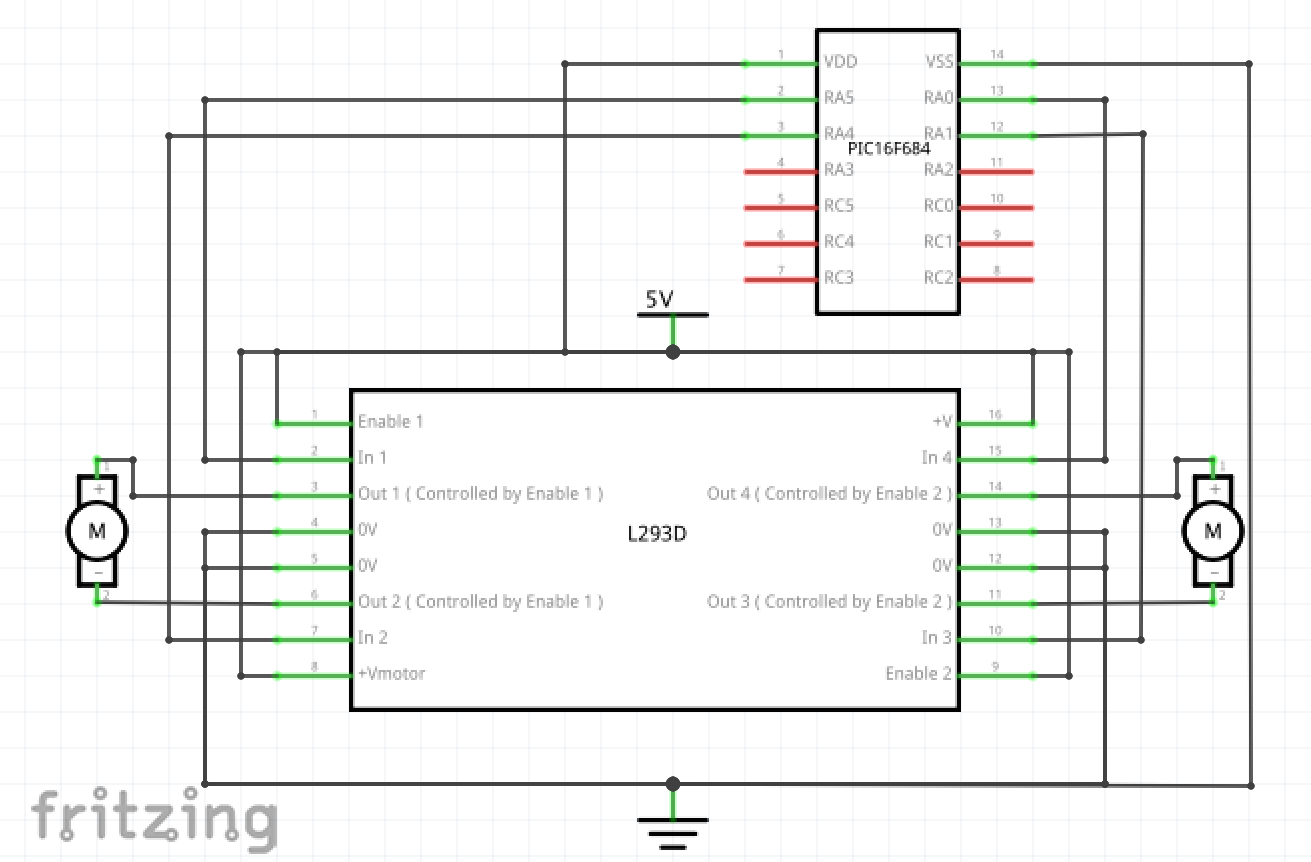
\includegraphics[width=10cm]{CircuitDiagram}
	\caption{The circuit diagram shown above does not include the circuit for the QRD1114 light sensors.}
	\end{SCfigure}
\subsection{Final Code}
\textit{Please refer to document within the main directory of this report for .txt code file.}
\end{document}          
